\chapter{Supporting software}

\subsection{Training dashboard}

To offer visibility into the training process. A GUI dashboard using Python library Rerun \sidecite{Rerun}. The dashboard allows real time inspection of the training process. A plot of training and validation loss. And most importantly, presents the latent learned latent profiles. Also offers a way to see prediction results for random slice out of validation dataset.

\begin{figure}[hb]
    \begin{tabular}{cc}
        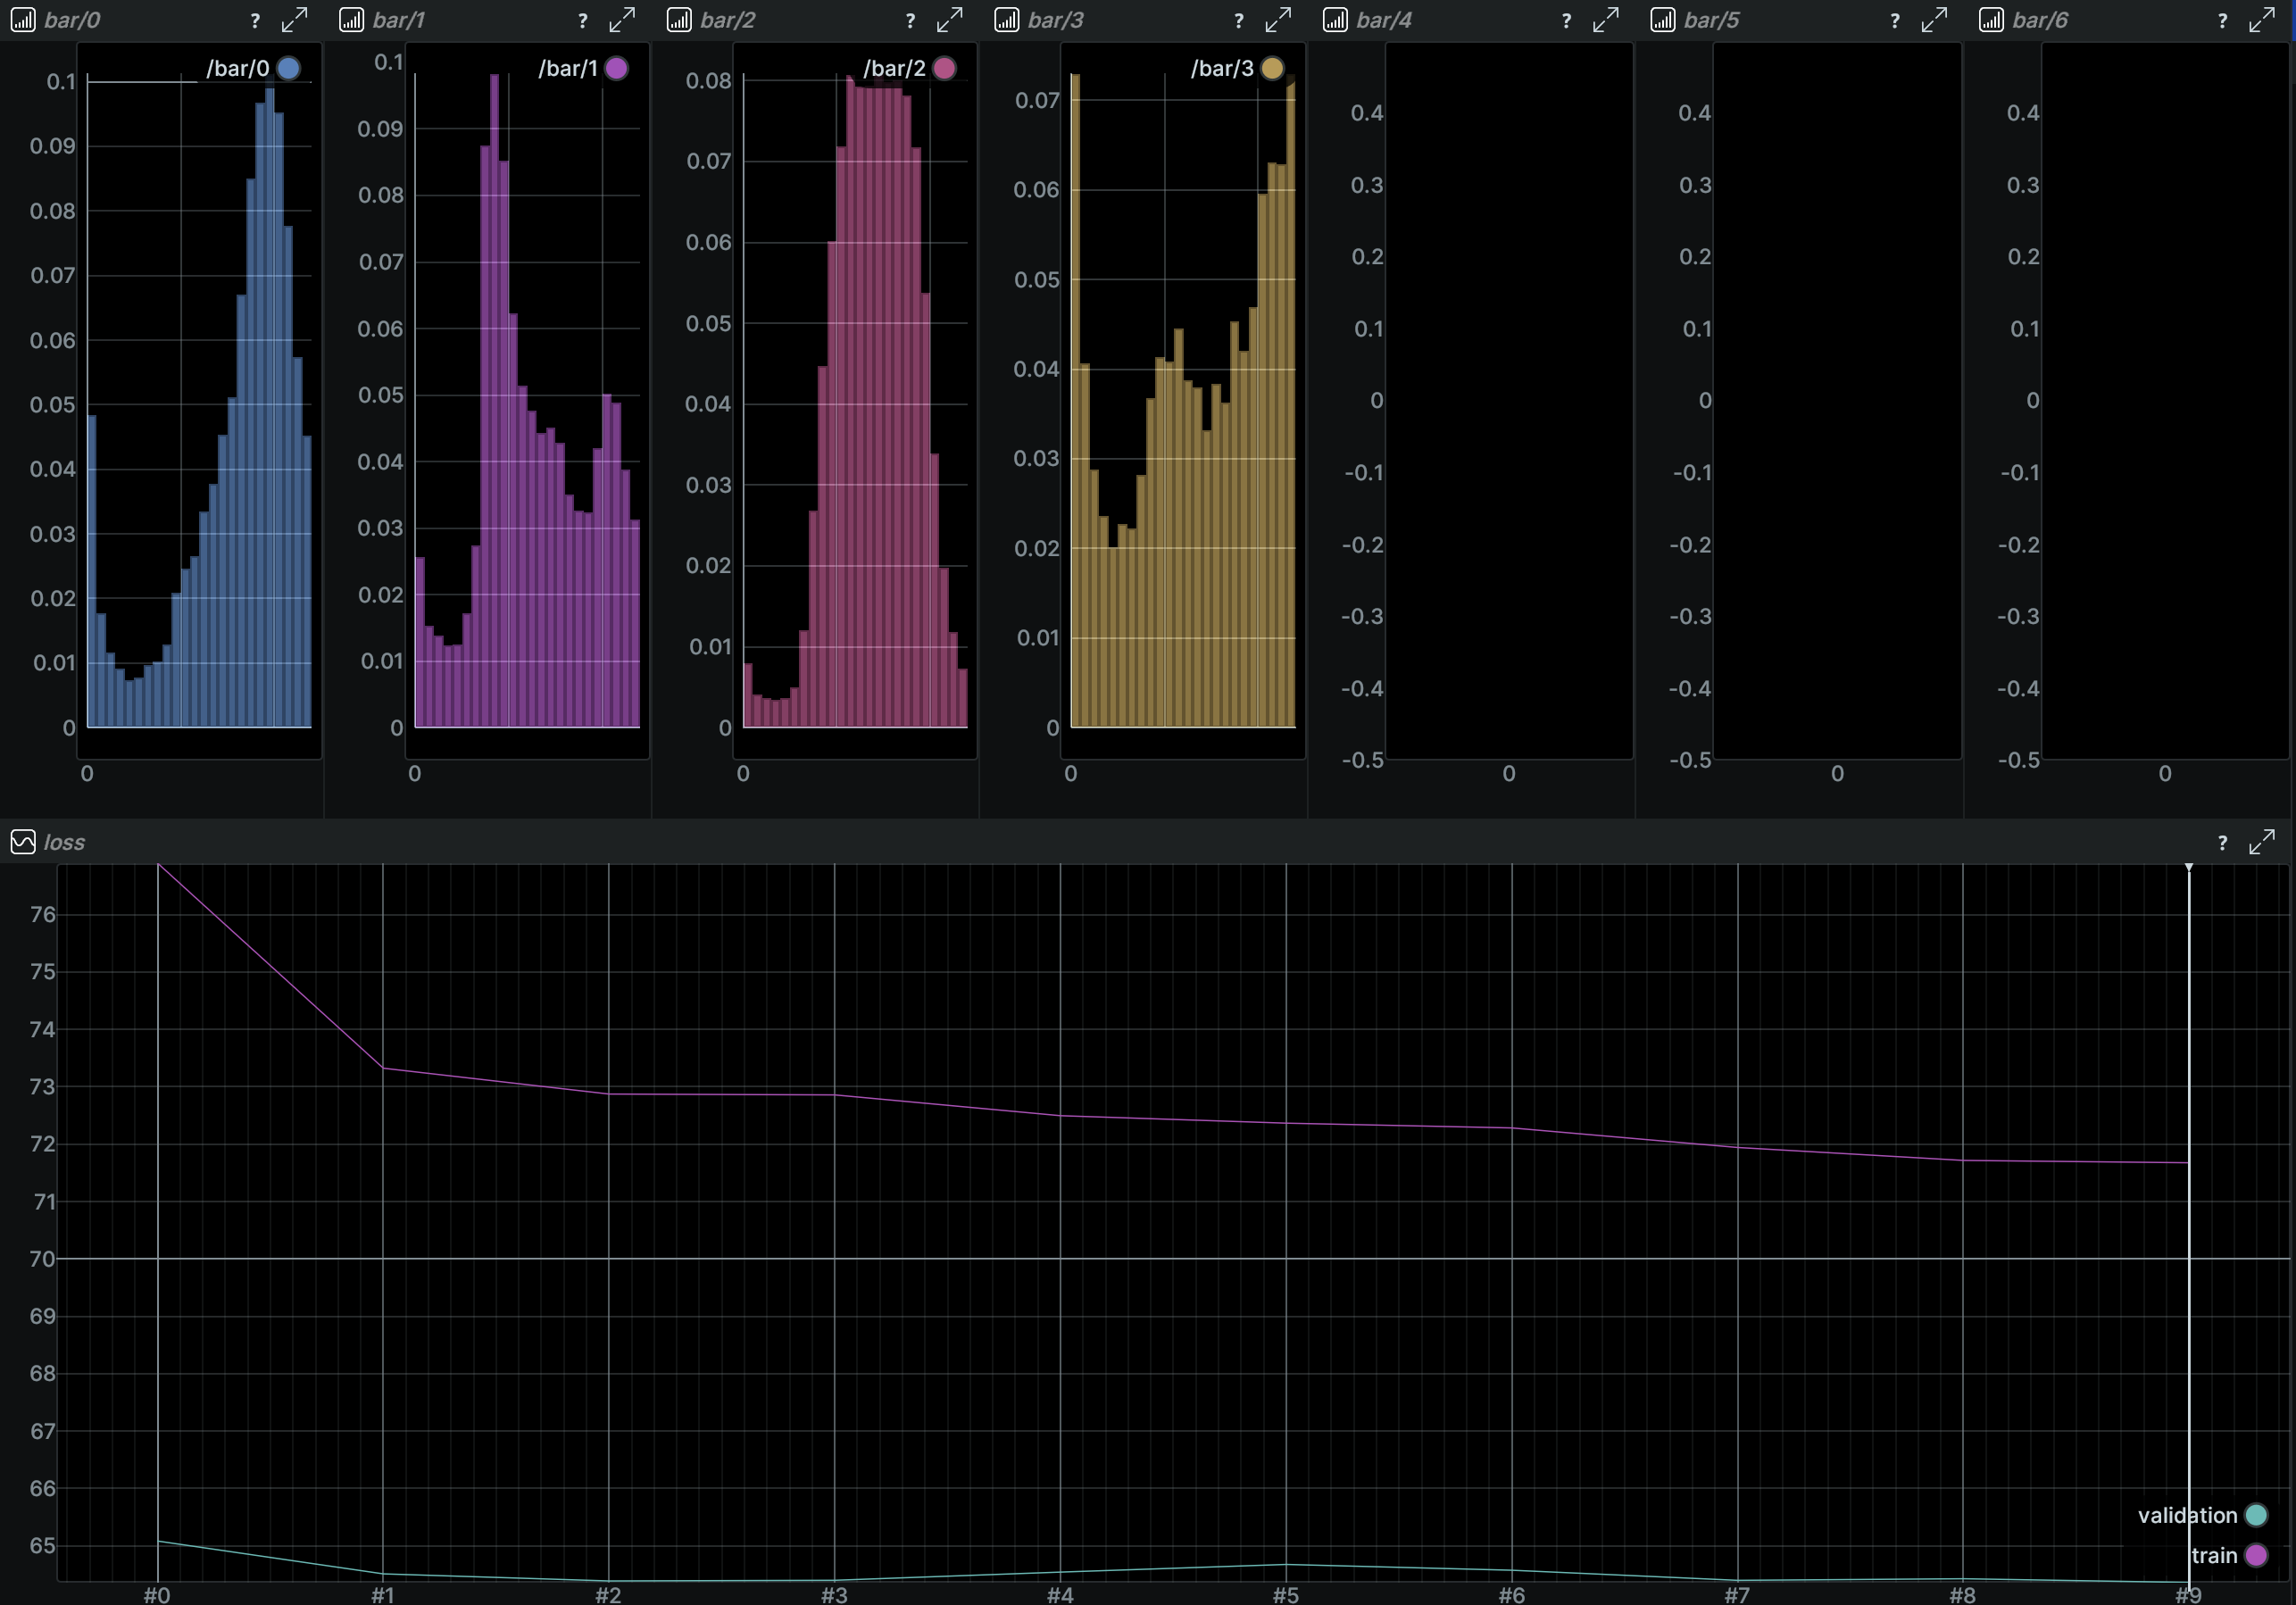
\includegraphics[width=0.7\textwidth]{rerun-train-validation.png} &
        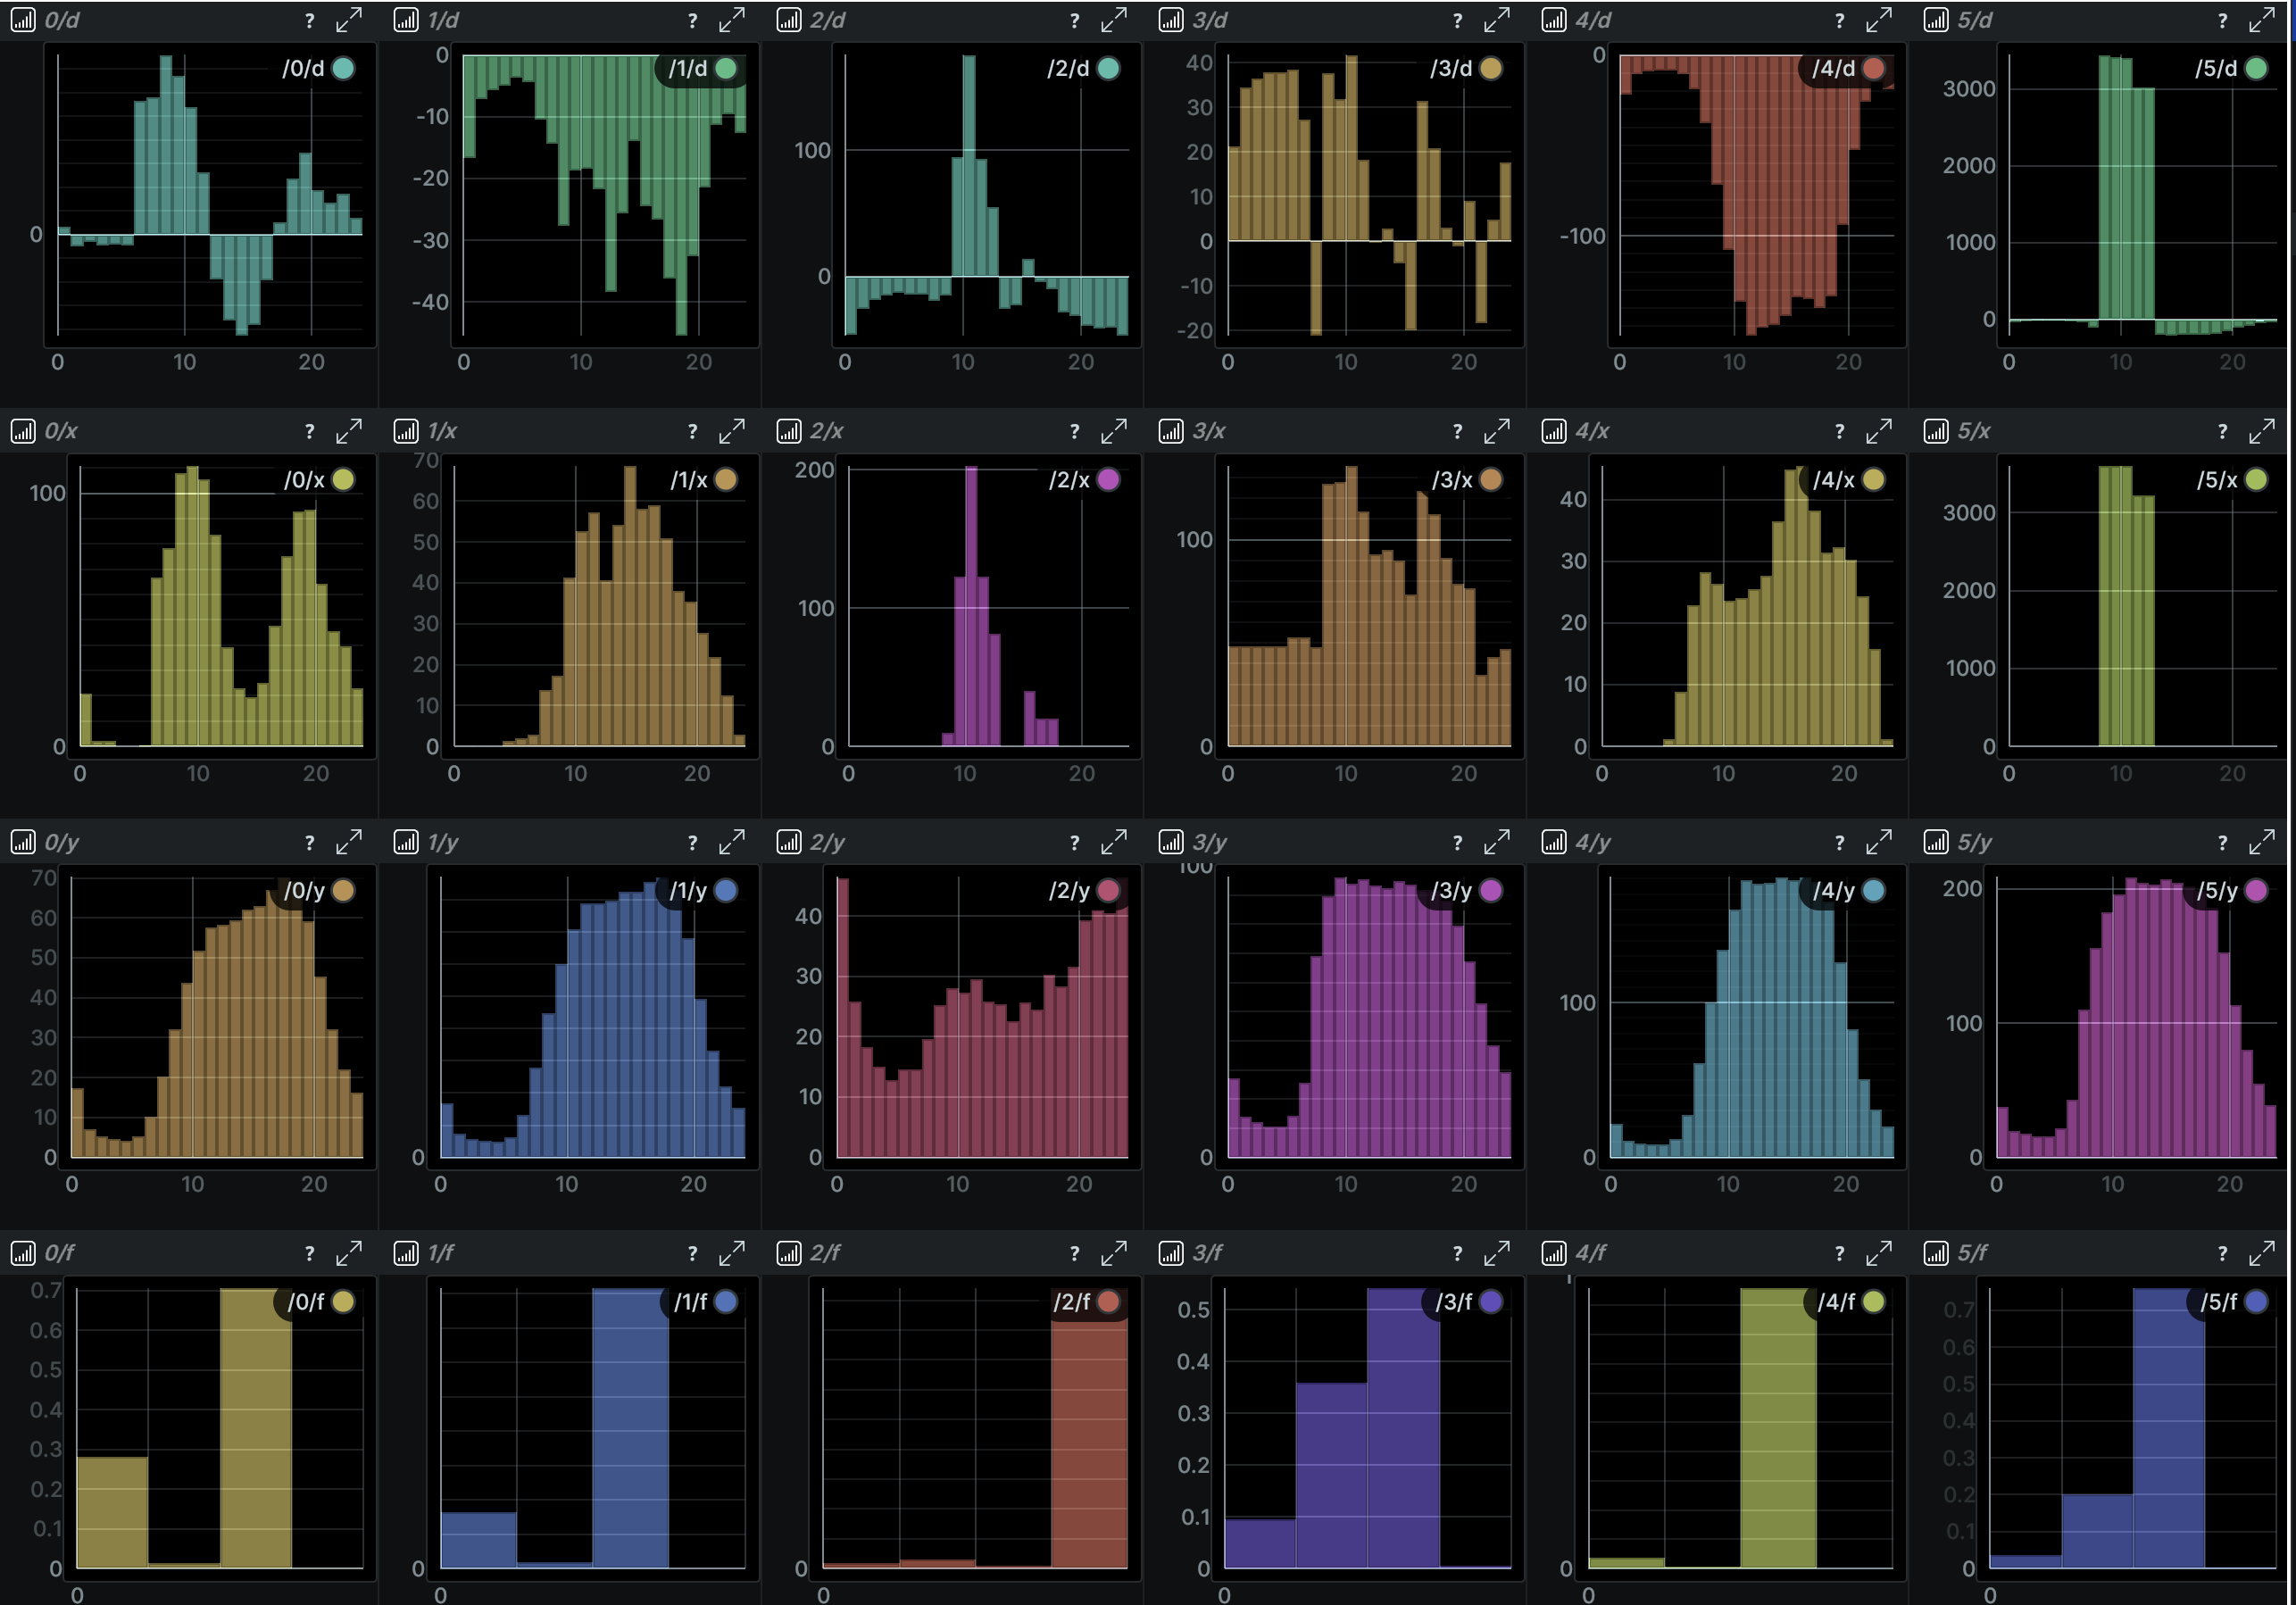
\includegraphics[width=0.7\textwidth]{rerun-predictions.png}
    \end{tabular}
    \caption{}{Rerun visualization dashboard.}
\end{figure}


\section{Tool for visualisation of prediction results}
To be able to inspect the prediction results in spatial context a tool was also developed with use of Streamlit\sidecite{StreamlitFasterWay2021}. The dashboard is in a form of a web application.
It consists of two screens.
First one allows inspection of overall model losses as visible in \ref{sec:res-comparison}. In bar charts and tabular formats. Where the bar chart shows all the types of losses relatively to each other.
\begin{figure}
    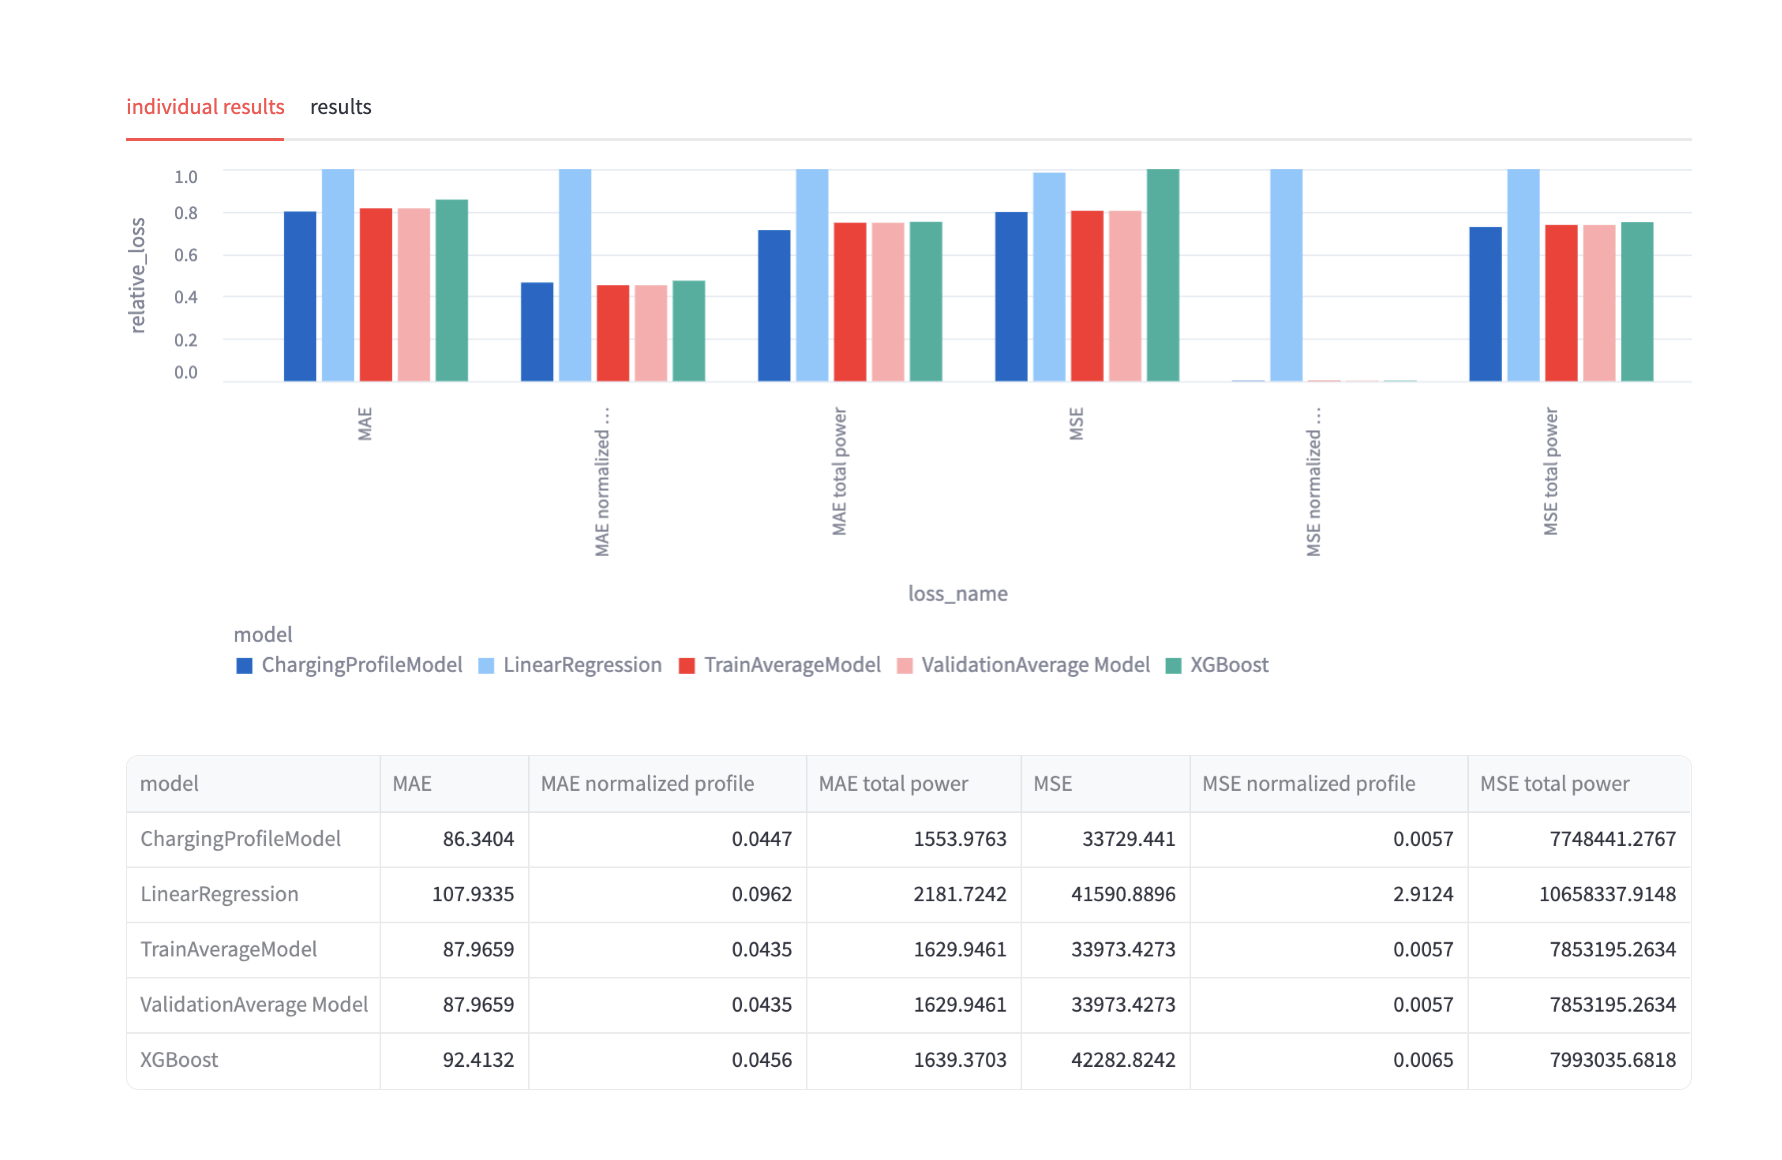
\includegraphics{data-dashboard-losses.png}
    \caption[]{Data dashboard website showing bar chart with relative losses of the models}
    \labfig{dasboard-all}
\end{figure}

The second screen displays table of all charging location together with day of the week and month. The individual rows of the table are selectable. When selection haapens location of the charger in map is shown and prediction from the model together with other models used for comparison is computed and its results are shown in a bar chart graph. Together with losses agains the original label $y$ value.

\begin{figure}
    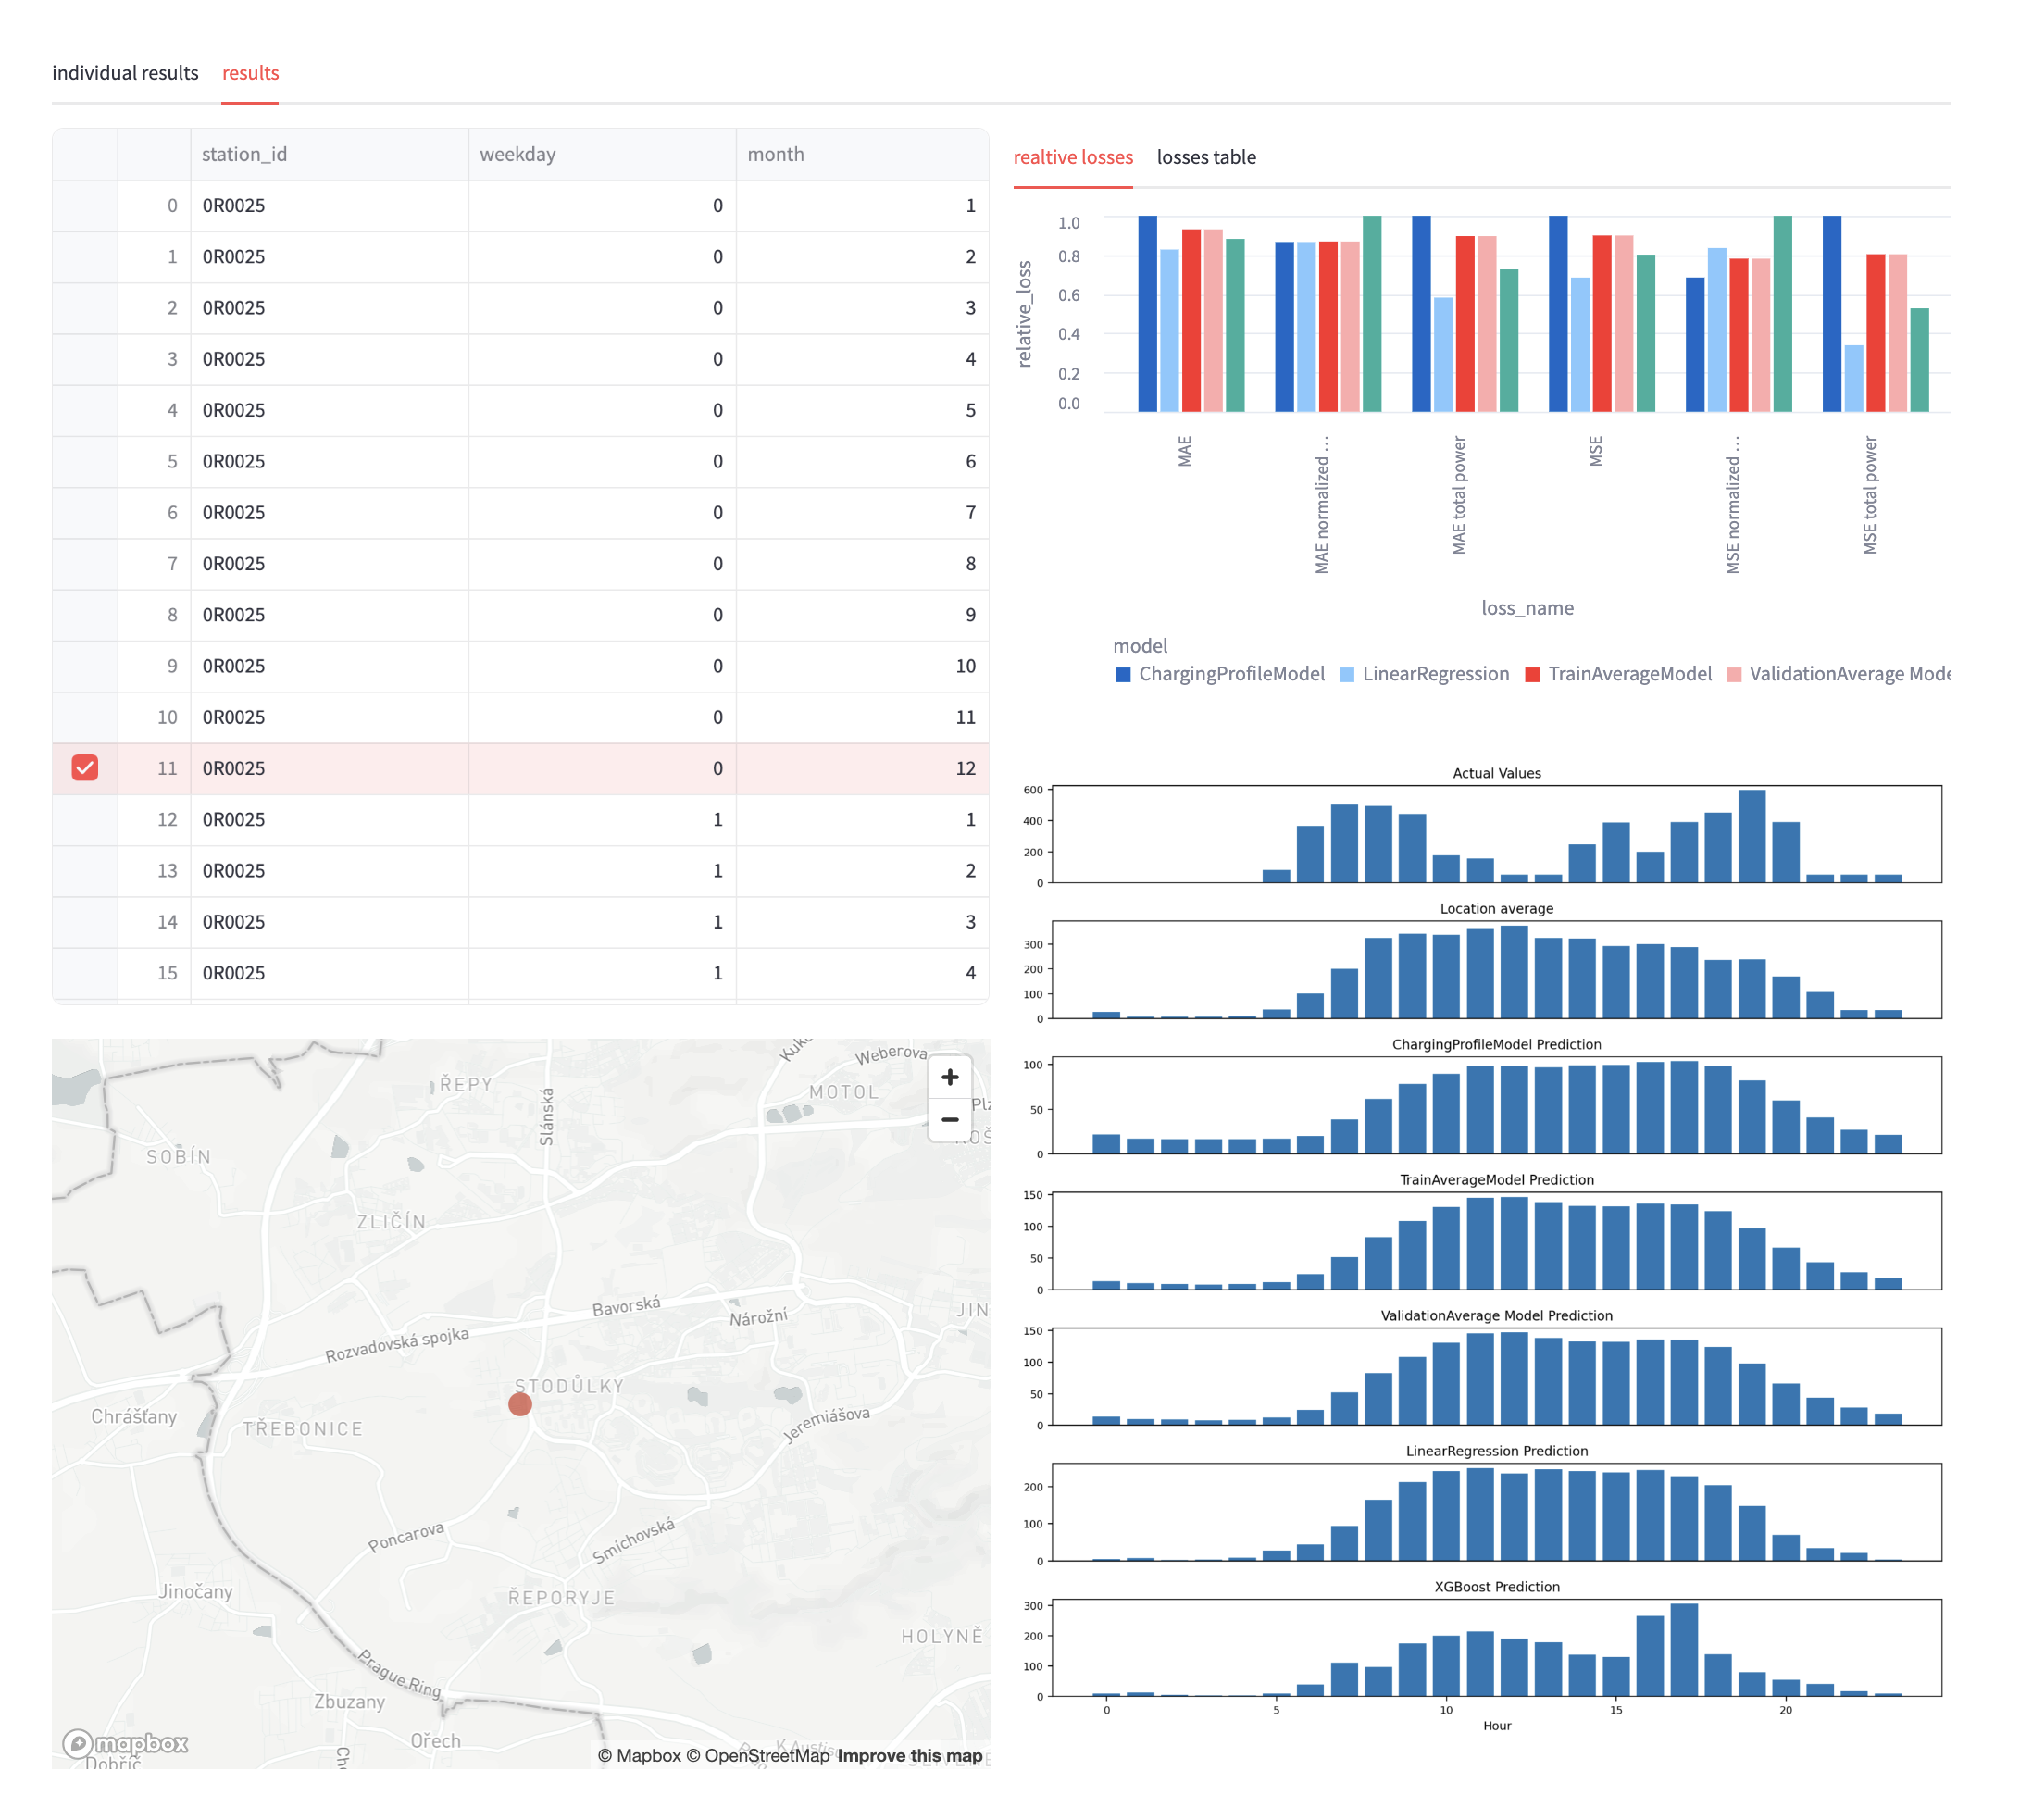
\includegraphics{data-dashboard-individual-predictions.png}
    \caption[]{Data dashboard website showing table with data from validation data set with one selected row. Of which the prediction is computed from the main model and the other models for comparison.}
    \labfig{dasboard-individual}
\end{figure}